\documentclass{article}
\usepackage{amsmath,amsfonts,amssymb,graphicx,color,float}
\begin{document}
\section*{3 JDemetra+ seasonal adjustment procedure}
\subsection*{\small 3.1 Schipol airport time series}
The time series used for this case study represents the air passenger movements registered at the Schipol airport in Amsterdam, the Netherlands. The series covers a length of 196 monthly registrations, spanning the period from January 1999 to April 2015. As visible from figure 5, which represents the unadjusted series, the data present a strong seasonal pattern, which is slightly varying over the entire series.
\begin{figure}[H]
\centering
  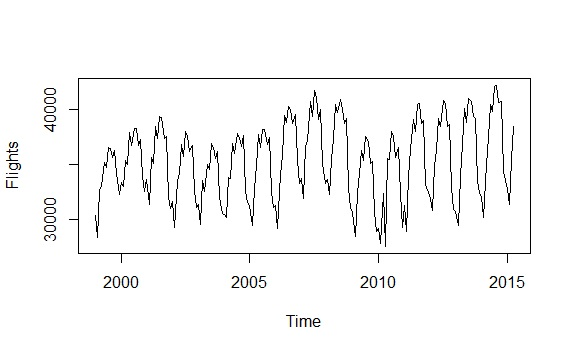
\includegraphics[width=\linewidth]{series.jpg}
  {\textbf{\scriptsize Figure 5: Amsterdam Schipol airport flights from January 1999 to April 2015}}
  \label{fig:1}
\end{figure}
\subsection*{\small 3.2 JDemetra+ introduction}
The first step is to carry out a seasonal adjustment with the tools included in JDemetra+, i.e. with TRAMO/SEATS and X-13-ARIMA procedures, without any pre-filtering treatment of the series. The software offers the possibility, through its \textit{workspace} window, to choose between different pre-defined \textit{specifications} implemented in the two methods. Those \textit{specifications} are sets of parameters and values assigned to them that contain all information necessary for seasonal adjustment and for modelling the time series during the pre-decomposition step. In table 2 are reported all the possible specifications (the first seven are from TRAMO/SEATS, the last six from X-13-ARIMA), but it is important to highlight two main points. First, the user has the option to set those parameters at will, depending on the nature of the analysis. Second, this paper will focus on the default specification settled by JDemetra+; \textit{RSAful}l for TRAMO/SEATS and \textit{RSA4c} for X-13-ARIMA, but with a fix model parameters choice, the so called ARIMA airline model (0,1,1)(0,1,1) (Box and Jenkins, 1976), one of the most commonly used seasonal ARIMA models, in order to meet the parsimony principle. The `Transformation' column indicates the performance of a test to choose between an additive decomposition (no transformation) and multiplicative decomposition (logarithmic transformation) of the time series. Concerning the ARIMA model selection, the acronym AMI stands for Automatic Model Identification. A detailed discussion of different parameters and specifications can be found in Grudkowska (2015).
\begin{figure}[H]
\centering
  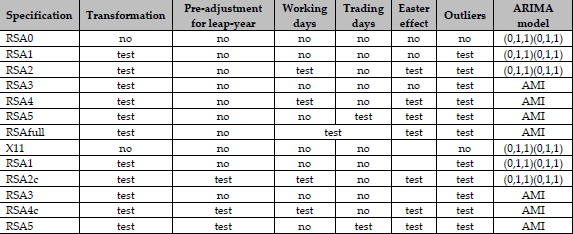
\includegraphics[width=\linewidth]{specification.jpg}
  {\textbf{\scriptsize Table 2: TRAMO/SEATS and X-13-ARIMA pre-defined specifications. }}
\end{figure}
The software performs an automatic identification of the calendar effects of a time series, and includes them as regressors in the RegARIMA model fitted in the \textit{modelling} step. This paper will not offer a thorough discussion about these regression parameters, i.e. outliers, Easter effect, trading/working days effect, leap-year effect; for it will mainly focuses about the Fourier-domain representation of the historical data. A useful discussion of the trading days effect identification and its spectral diagnostic is offered by Findley \& Soukup (1999). In this case study, the parameters selection procedure will not be modified from the automatic one performed by the software.
\subsection*{\small 3.3 JDemetra+ spectral analysis}
A helpful tool implemented in JDemetra+ refers to the spectral analysis of time series. The possibilities for a spectral analysis within the software are Periodogram, Auto-regressive Spectrum and Tukey Spectrum. The study will focus only on the periodogram. Figure 6 presents the periodogram of the analysed data. As mentioned in the section 2.3, this periodogram considers a first difference operation on data. As in most of the JDemetra+ tools, users are free to change this parameter, increasing the differencing order or annulling it. JDemetra+ points out the significance of a peak through a green horizontal line, which denotes the 0.05 significance level.
\begin{figure}[H]
\centering
  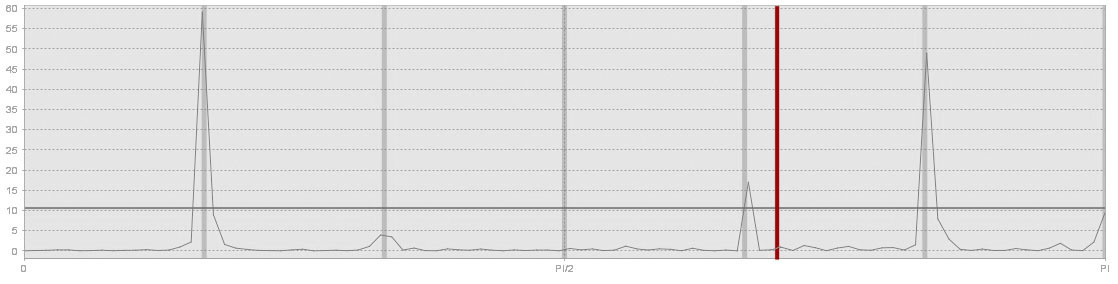
\includegraphics[width=\linewidth]{amsper.jpg}
  {\textbf{\scriptsize Figure 6: Periodogram of unadjusted time series}}
  \label{fig:1}
\end{figure}
The unadjusted series shows a peak at the first seasonal frequency, which means the presence of a strong seasonal movement of one cycle per year. Another significant peak coincides with the fifth seasonal frequency, related to a movement of five cycles per year. This periodogram gives results which could be visible also from the simple plot of the series (the presence of seasonality), but from this frequency-domain representation it is more straightforward to check the cycles of the dominant seasonal movements.\\When starting a seasonal adjustment with JDemetra+, both the methods imply two steps; a \textit{modelling} part and a \textit{decomposition} part. As briefly discussed in the first chapter, the \textit{modelling} part takes care, first, of identifying the regression parameters that have a deterministic effect on the data; and second, of fitting an ARIMA model to the data, in order to give a suitable model for an acceptable decomposition. Since this paper focuses on the designed filter to decompose a time series in its components, there is no detailed discussion of the \textit{modelling} results, but rather on the spectral diagnostics of the decomposition output and the filtering procedures. Indeed, JDemetra+ offers several diagnostics, using a user-friendly graphic for the results of the various tests. Together with every \textit{p.value} associated to each test, a description of the result is given in words (good, uncertain, bad) coloured, respectively, in green, yellow and red. This helps for interpretation of the results.
\subsection*{\small 3.4 TRAMO/SEATS and X-13-ARIMA spectral diagnostics}
Once the seasonal adjustment has been performed, JDemetra+ evaluates the quality of the decomposition through a wide range of diagnostics. Within these, a \textit{spectral diagnostic} consists in three frequency-domain charts, one for the model residuals, one for the irregular component, and one for the seasonally adjusted series. Actually, the software offers these diagnostics both as periodogram and as auto-regressive spectrum, but only the periodograms are considered here. Figure 7 plots the periodogram of the residuals. A peak in this periodogram at seasonal or trading day frequencies indicates the need for fitting a better model. In particular, peaks at seasonal frequencies suggests a different filter choice for the decomposition, while peaks at the trading day frequency suggests the inappropriate choice of regression variables used in the model.
\begin{figure}[H]
\centering
  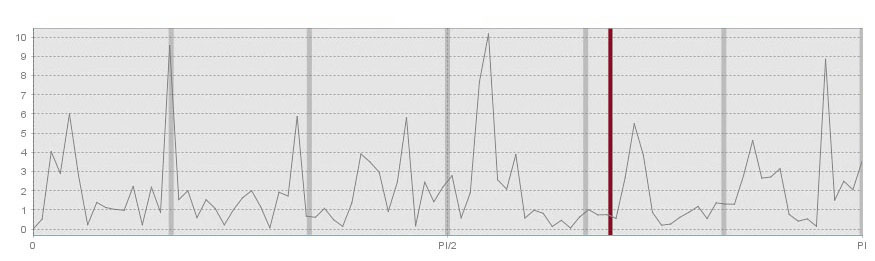
\includegraphics[width=\linewidth]{perRES.jpg}
  {\textbf{\scriptsize Figure 7: TRAMO/SEATS residuals periodogram.}}
  \label{fig:1}
\end{figure}
In the periodogram of residuals obtained from the TRAMO/SEATS method no peak exceeds the significance level, even if some movements is present through different frequencies; particularly, a peak is visible at the first seasonal frequency. A peak in the spectrum of the seasonally adjusted series or irregulars reveals inadequacy of the seasonal adjustment filters for the time interval used for spectrum estimation. In this case different model specification or data span length should be considered.
\begin{figure}[H]
  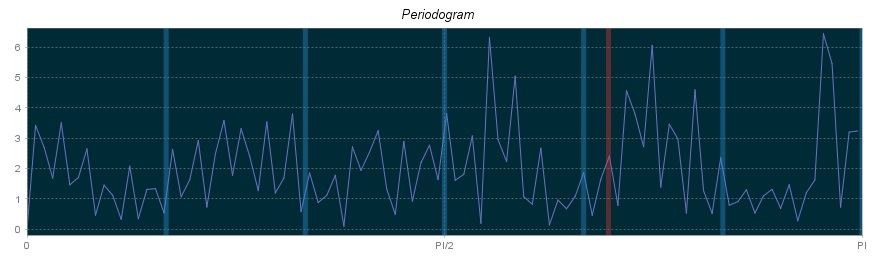
\includegraphics[width=\linewidth]{perIRR.jpg}
\end{figure}
\begin{figure}[H]
\centering
  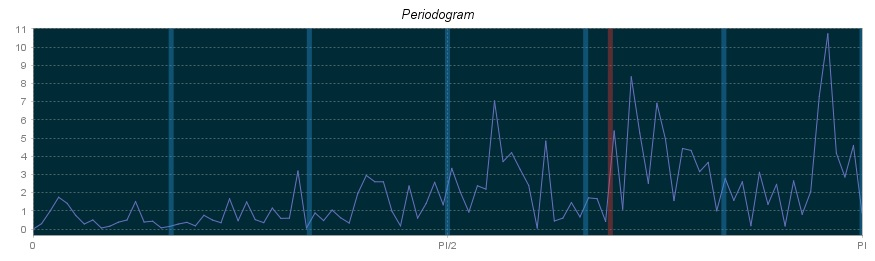
\includegraphics[width=\linewidth]{perSA.jpg}
  {\textbf{\scriptsize Figure 8: TRAMO/SEATS irregular and seasonally adjusted series periodogram.}}
\end{figure}
For computational reasons, in JDemetra+, none of the periodograms for seasonally adjusted series and for the irregular displays the line that highlights peaks above the 0.05 significance level. In the adjusted series (figure 8 lower chart), the periodogram does not show any peak at seasonal frequencies, attesting a good decomposition of the original series performed by SEATS and a satisfactory removal of the seasonal effect. As desirable, low frequencies have low amplitudes, while higher values are registered at higher frequencies, in between the seasonal harmonics. Indeed, the noise component is not totally removed, as can be seen in the upper chart of figure 8, related to the irregular periodogram, which shows relevant power between seasonal frequencies. In the next chapter about the adjustment of the filtered series, those same plots will show a much smoother behaviour. In the following charts are reported the same three periodograms, but the ones obtained from the X-13-ARIMA procedure, which makes the use of 3x3 seasonal filter and a 13-terms Henderson moving average as trend filter. The length of these filters depends on the time series, and the selection is done automatically by the X-11 algorithm (Dagum et al, 1996). For the comprehension of the length selection criterion, see Grudkowska (2015), while a brief discussion of how these filters work will be provided in the appendix. These periodograms, in figure 9, show a similar behaviour to the ones obtained from TRAMO/SEATS, and their interpretation is the same. 
\begin{figure}[H]
  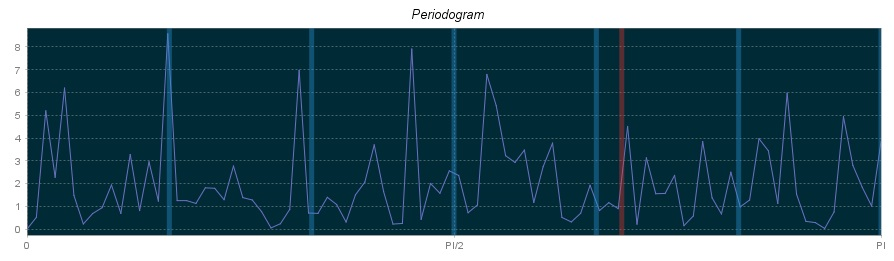
\includegraphics[width=\linewidth]{XperRES.jpg} 
  \label{fig:1}
\end{figure}
\begin{figure}[H]
  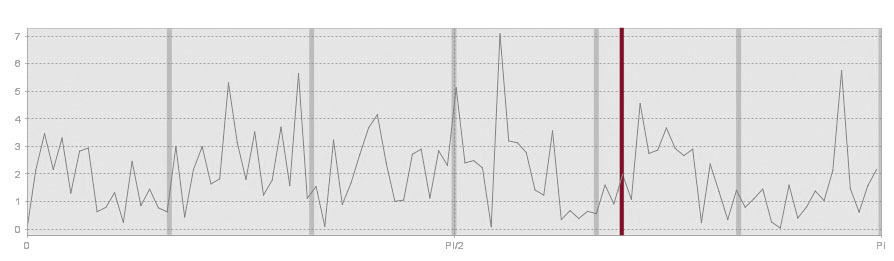
\includegraphics[width=\linewidth]{XperIRR.jpg} 
  \label{fig:1}
\end{figure}
\begin{figure}[H]
  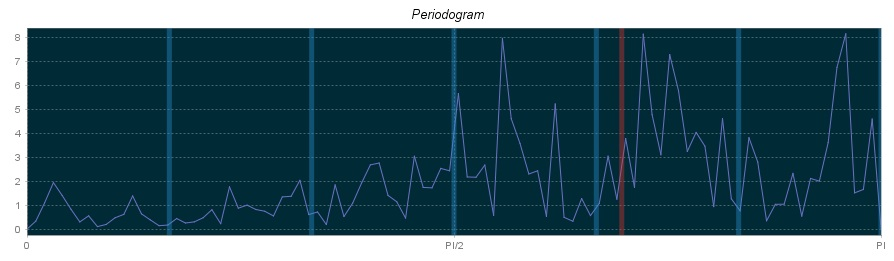
\includegraphics[width=\linewidth]{XperSA.jpg} 
   {\textbf{\scriptsize Figure 9:  X-13-ARIMA residuals, irregular and seasonally adjusted series periodogram. }}
  \label{fig:1}
\end{figure}
\subsection*{\small 3.5 Squared gain of components filter}
TRAMO/SEATS estimates the various components using the so-called Wiener-Kolmogorov filters. These filters are symmetric; it means that observation from the past and the future for every observation have to exist, so there is the need for forecast and backcasts for both ends of the series. This operation is performed through the ARIMA model estimated by TRAMO.  An interesting tool regarding the quality of the decomposition is the square gain of the components filter. This indicates which frequency component are suppressed or amplified by the filter, i.e. it controls which movement of particular amplitude at a frequency $\omega$ is delivered to the output series. For monthly data, the squared gain function of the filter is the amplitude function of its transfer function. If in a frequency band [$\omega_{1};\omega_{2}$] the squared gain has value zero, then the output series is free of movements in that range; if is equal to one, all the movements from that range is passed on to the component estimator. It means that the seasonal component estimator is expected to capture only the seasonal frequencies (taking unitary values at these frequencies), while the seasonally adjusted series estimator should have zero at these same frequencies, in order to eliminate the seasonal effects. In general, the squared gain shape depends on the model for the time series. A thorough explanation of the derivation of the squared gain and its interpretation, as the parameter values of the ARIMA model and the length T of the series change, is discussed in Findley \& Martin (2006).
\begin{figure}[H]
\centering
  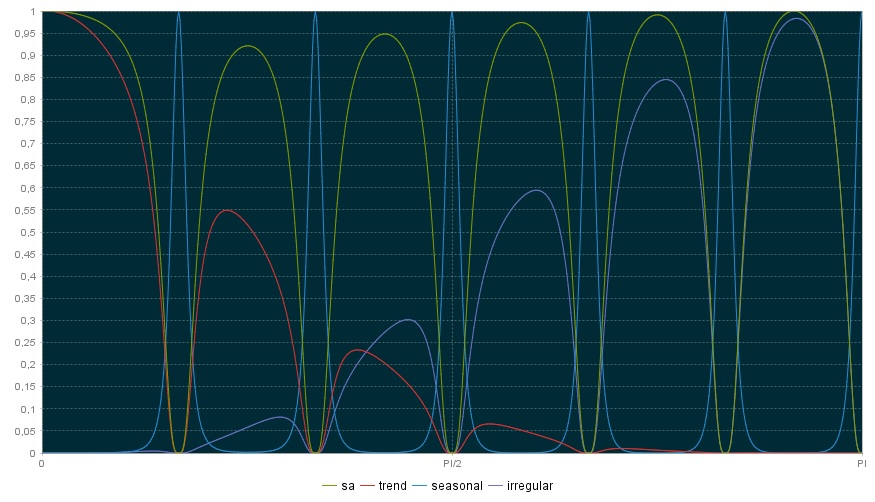
\includegraphics[width=\linewidth]{squaredgain.jpg}
  {\textbf{\scriptsize Figure 10: Squared gain of TRAMO/SEATS components filter}}
\end{figure}
Figure 10 represent the squared gain of the components filter obtained by TRAMO/SEATS from the data set analysed in here. As the value for seasonal component estimator is equal to one at seasonal frequencies, the decomposition procedure seems to act pretty well, with relatively narrow troughs. On the other hand, the shape of the squared gain of the seasonally adjusted component filter seems to miss some signal between seasonal frequencies, and it doesn't reach the exact value of one. It will be interesting, in the next chapter, to compare this squared gain chart to the one obtained from the same data pre-filtered through the designed filter.
As X-13-ARIMA makes use of the algorithm of X-11, which implies the use of standard filters (seasonal moving average and Henderson filters, where only the filter length may vary), JDemetra+ doesn't offer a squared gain representation of these filters, but only for the TRAMO/SEATS ones, since they are defined differently for each analysed time series.
\end{document}